\subsection{The Selection of Cities}

We collect data on five cohorts of individuals raised in Reggio Emilia, Parma, and Padova. Parma and Padova are similar to Reggio Emilia in terms of size, geographic, demographic, and socio-economic structure, but they do not have the Reggio Approach available.\footnote{Other Italian cities were taken into consideration, notably Brescia, Livorno, Modena, Perugia, Piacenza, Prato, and Ravenna. Parma and Padova were the two cities that best fulfilled our comparability and sample requirements.} 

We collect demographic data to explore the similarities among the three cities. Reggio Emilia has a population of roughly 173,000, Parma of 188,000, and Padova of 210,000 in 2013.\footnote{The population size in December 2013 was 172,525 in Reggio Emilia, 187,938 in Parma, and 209,678 in Padova. Source: ISTAT, \url{http://www.demo.istat.it/}} Figure \ref{fig:population} shows the similar rising trends in population in three cities. 

Also their economic resources are comparable: Reggio Emilia has an average per-capita income of 25,226 euros, Parma of 28,437, and Padova of 29,915 in 2011.\footnote{Source: Finance Minister, taxable income for 2011.}
%See \url{http://www.comuni-italiani.it/statistiche/redditir2011.html}

Even more importantly, these three cities face analogous fertility dynamics and, consequently, potential demand for child-care services. Figure~\ref{fig:population} shows that three cities observe similar trend in birth rate and natural rate. Trends in migration are also similar in three cities, which is shown in Figure~\ref{fig:emigr-immigr}. Although emigration rate is highest in Padova and net migration rate is highest in Reggio for most of the years, general trends in emigration and immigration in similar in all cities. Trends in foreign migration are almost identical in three cities. Appendix~\ref{sec:data-app} presents more information on the characteristics of the three cities.

\begin{figure}[H]
      \centering
        \begin{subfigure}[t]{0.49\textwidth}
          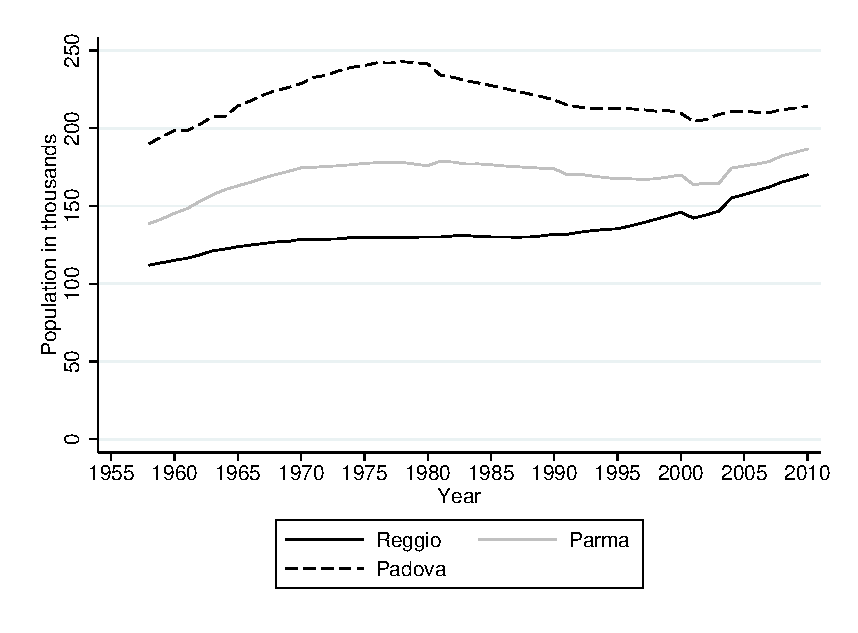
\includegraphics[width=\textwidth]{../../output/image/population.eps}
\caption{Population}
        \end{subfigure}
        \begin{subfigure}[t]{0.49\textwidth}
          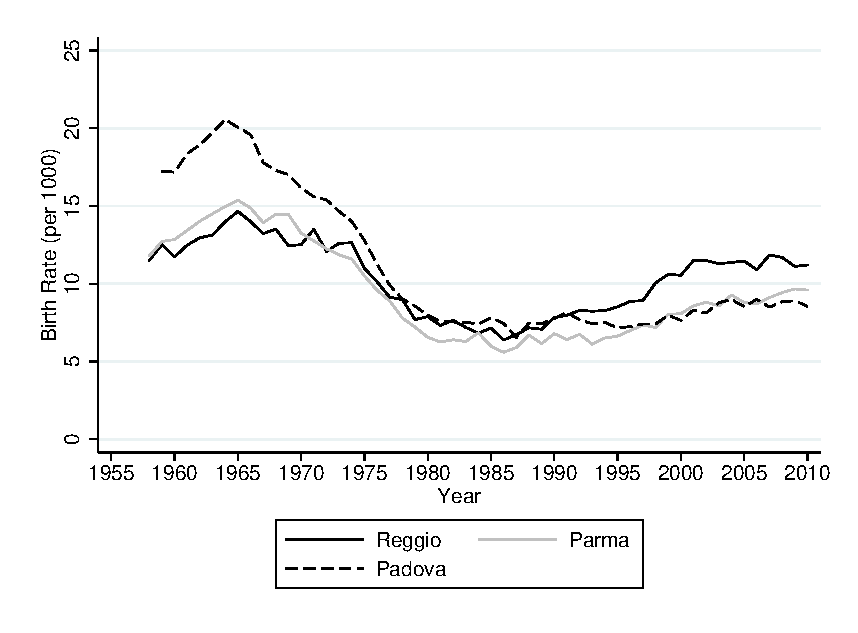
\includegraphics[width=\textwidth]{../../output/image/birth_rate.eps}
 \caption{Birth Rate}
        \end{subfigure}
        \begin{subfigure}[t]{0.49\textwidth}
          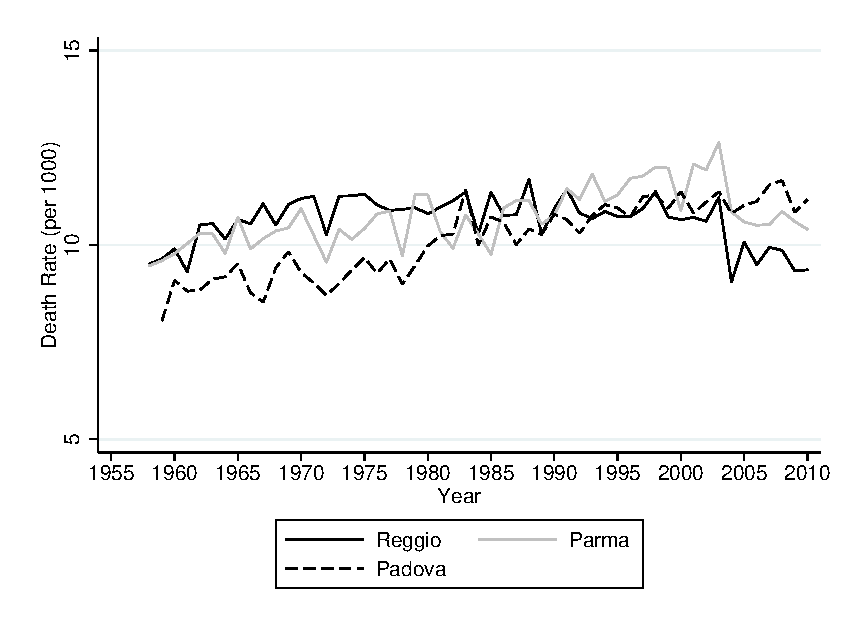
\includegraphics[width=\textwidth]{../../output/image/death_rate.eps}
        \caption{Death Rate}
        \end{subfigure}
        \begin{subfigure}[t]{0.49\textwidth}
          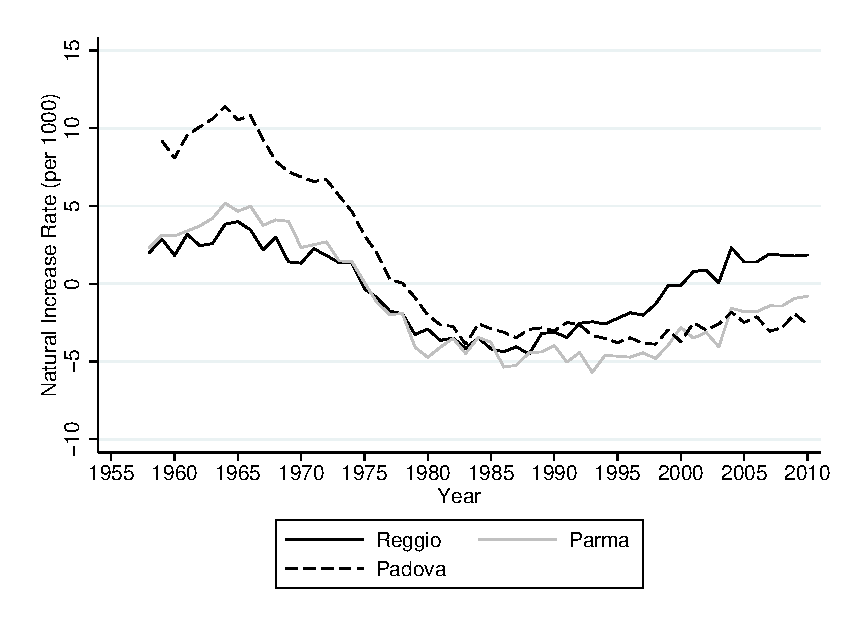
\includegraphics[width=\textwidth]{../../output/image/naturalinc_rate.eps}
            \caption{Natural Rate}
        \end{subfigure}
      \caption{Population Statistics}  \label{fig:population}
    \end{figure}

\textbf{[JJH: Can we test for equality across cities?]}

\begin{figure}[H]
      \centering
        \begin{subfigure}[t]{0.49\textwidth}
          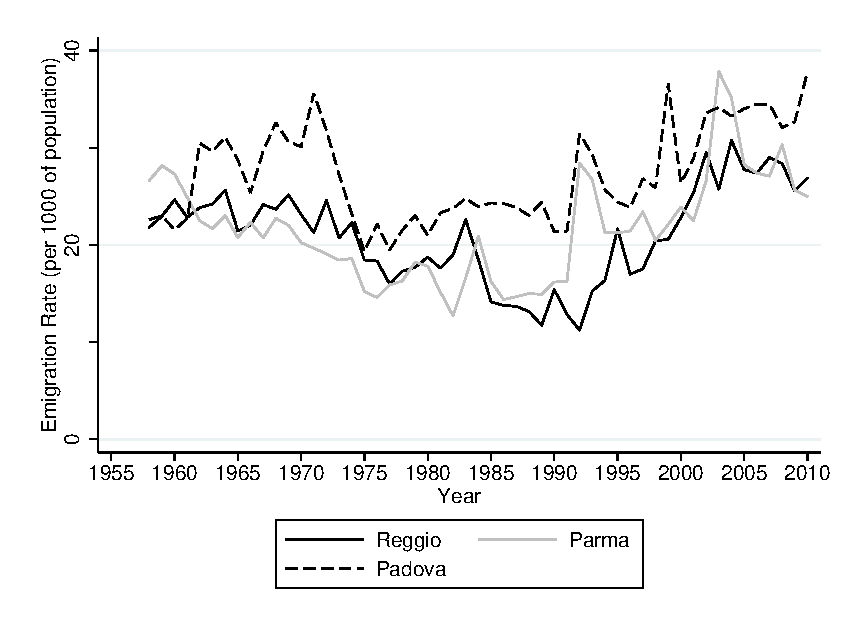
\includegraphics[width=\textwidth]{../../output/image/emigration.eps}
            \caption{Emigration}
        \end{subfigure}
      \begin{subfigure}[t]{0.49\textwidth}
        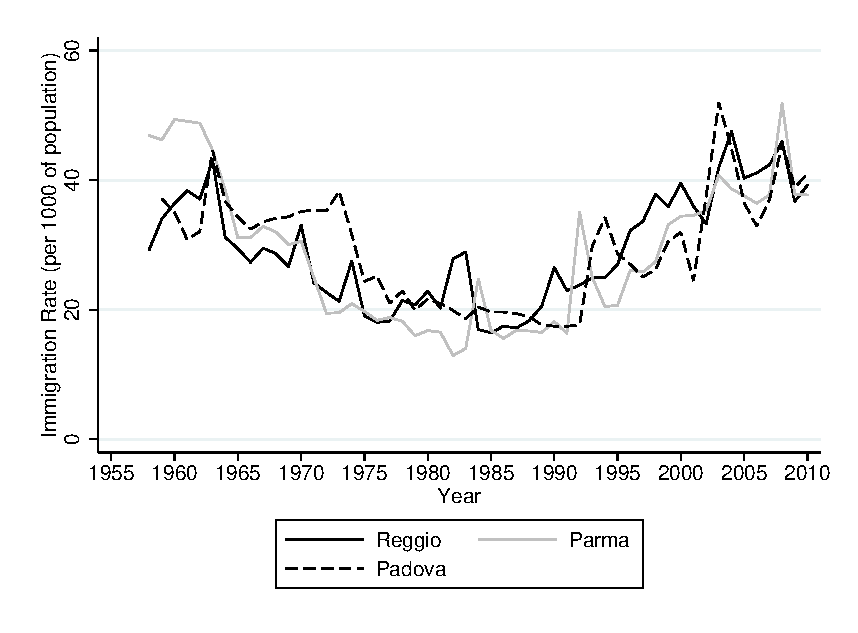
\includegraphics[width=\textwidth]{../../output/image/immigration.eps}
        \caption{Immigration}
      \end{subfigure}
	 \begin{subfigure}[t]{0.49\textwidth}
          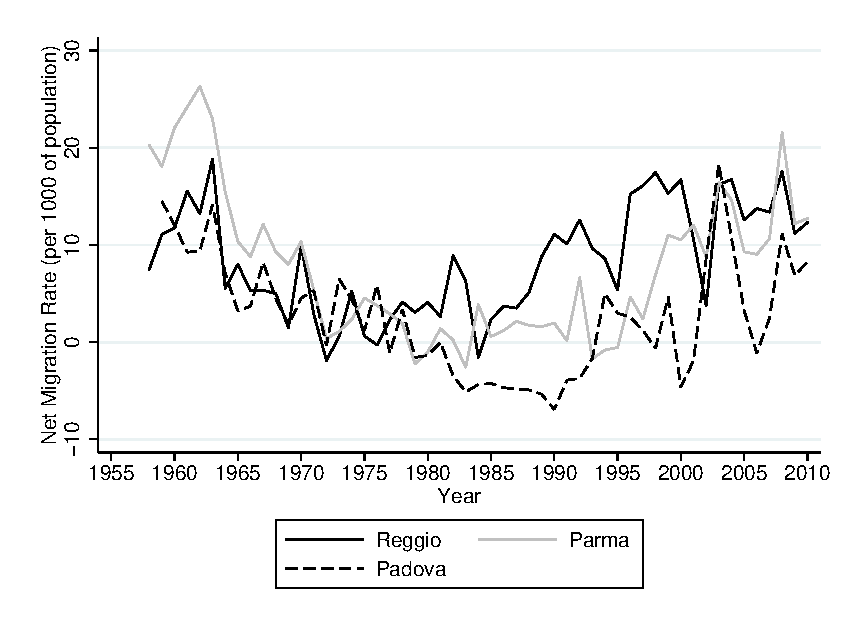
\includegraphics[width=\textwidth]{../../output/image/netmigration.eps}
\caption{Net Migration}
        \end{subfigure}
        \begin{subfigure}[t]{0.49\textwidth}
          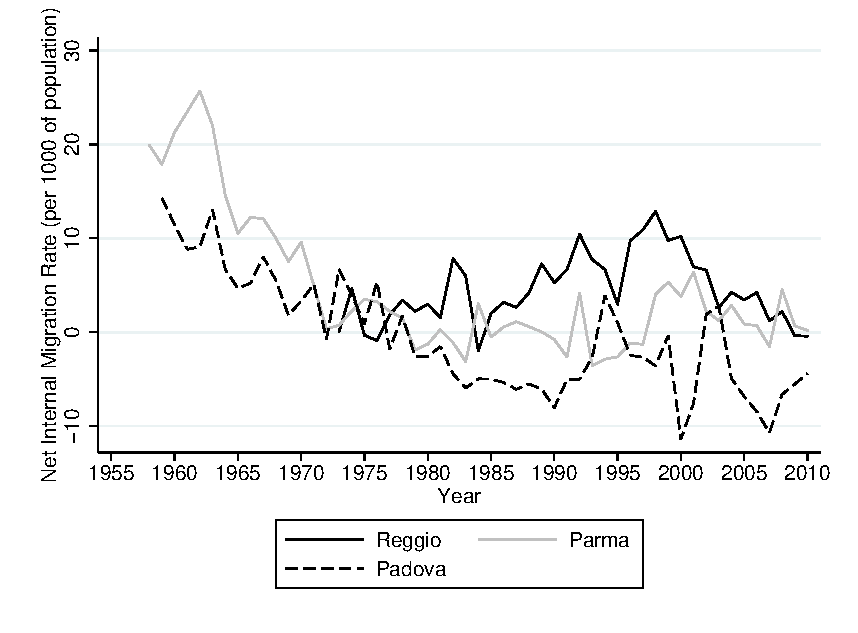
\includegraphics[width=\textwidth]{../../output/image/netinternalmig.eps}
 \caption{Net Internal Migration}
        \end{subfigure}
        \begin{subfigure}[ht]{0.48\textwidth}
          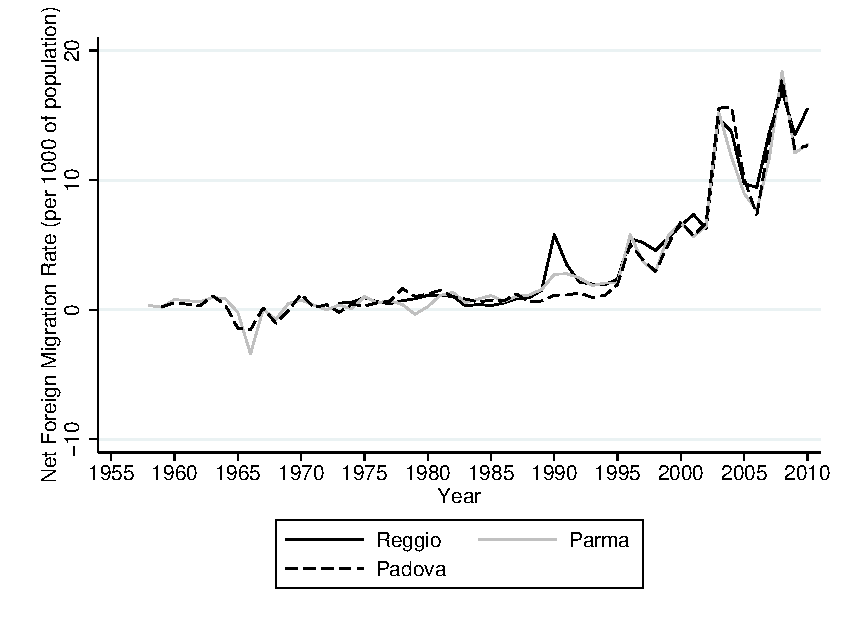
\includegraphics[width=\textwidth]{../../output/image/netforeignmig.eps}
        \caption{Net Foreign Migration}
        \end{subfigure}

      \caption{Migration Statistics}  \label{fig:emigr-immigr}
    \end{figure}